\section{SLTRs durch harmonische Funktionen}\label{harmonic_approach}

Zum Einstieg eine weitere Definition, die es ermöglicht eine Beobachtung zu SLTRs festzuhalten. Die Beweise zu den in diesem Abschnitt aufgestellten Propositionen und Theoremen werden ausgelassen. Sie befinden sich, wenn nicht anders angegeben, in der entsprechenden Arbeit von Aerts und Felsner \cite{af13}.

\begin{definition}[Begrenzende Zykel und kombinatorisch konvexe Ecken]\label{def_ccc}
Sei $G$ ein ebener Graph mit Aufhängungen $\{a_1,a_2,a_3\}$ und einem FAA $\phi$ von G. Sei $H$ ein zusammenhängender Teilgraph von G und $\gamma=\gamma(H)$ der H umrandende Weg in G. Somit ist $\gamma$ eine Folge aus Kanten und Knoten die $H$ in $G$ begrenzt. Knoten und Kanten können in $\gamma$ mehrfach vorkommen (vergleiche Abbildung \ref{corner_def}). Wir werden so erhaltene $\gamma$ als \textit{begrenzende Zykel} bezeichnen. Die Menge der Knoten, Kanten und Gebiete aus $G$, die im Inneren von $\gamma$ oder auf $\gamma$ liegen, bezeichnen wir mit int$(\gamma)$. Einen Knoten $v$ aus $\gamma$ bezeichnen wir als \textit{kombinatorisch konvexe Ecke} von $\gamma$ im Bezug auf $\phi$, falls gilt:
\begin{itemize}
\item [E1] $v$ ist eine Aufhängung, oder
\item [E2] $v$ ist nicht durch $\phi$ zugeordnet und es existiert eine Kante $e = (v,w)$ mit $e \notin int(\gamma)$, oder
\item [E3] $v$ ist einem Gebiet $f$ zugeordnet, $f \notin int(\gamma)$ und es existiert eine Kante $e = (v,w)$, sodass $e \notin int(\gamma)$.
\end{itemize}
\end{definition}

\begin{figure}[h]
	\centering
  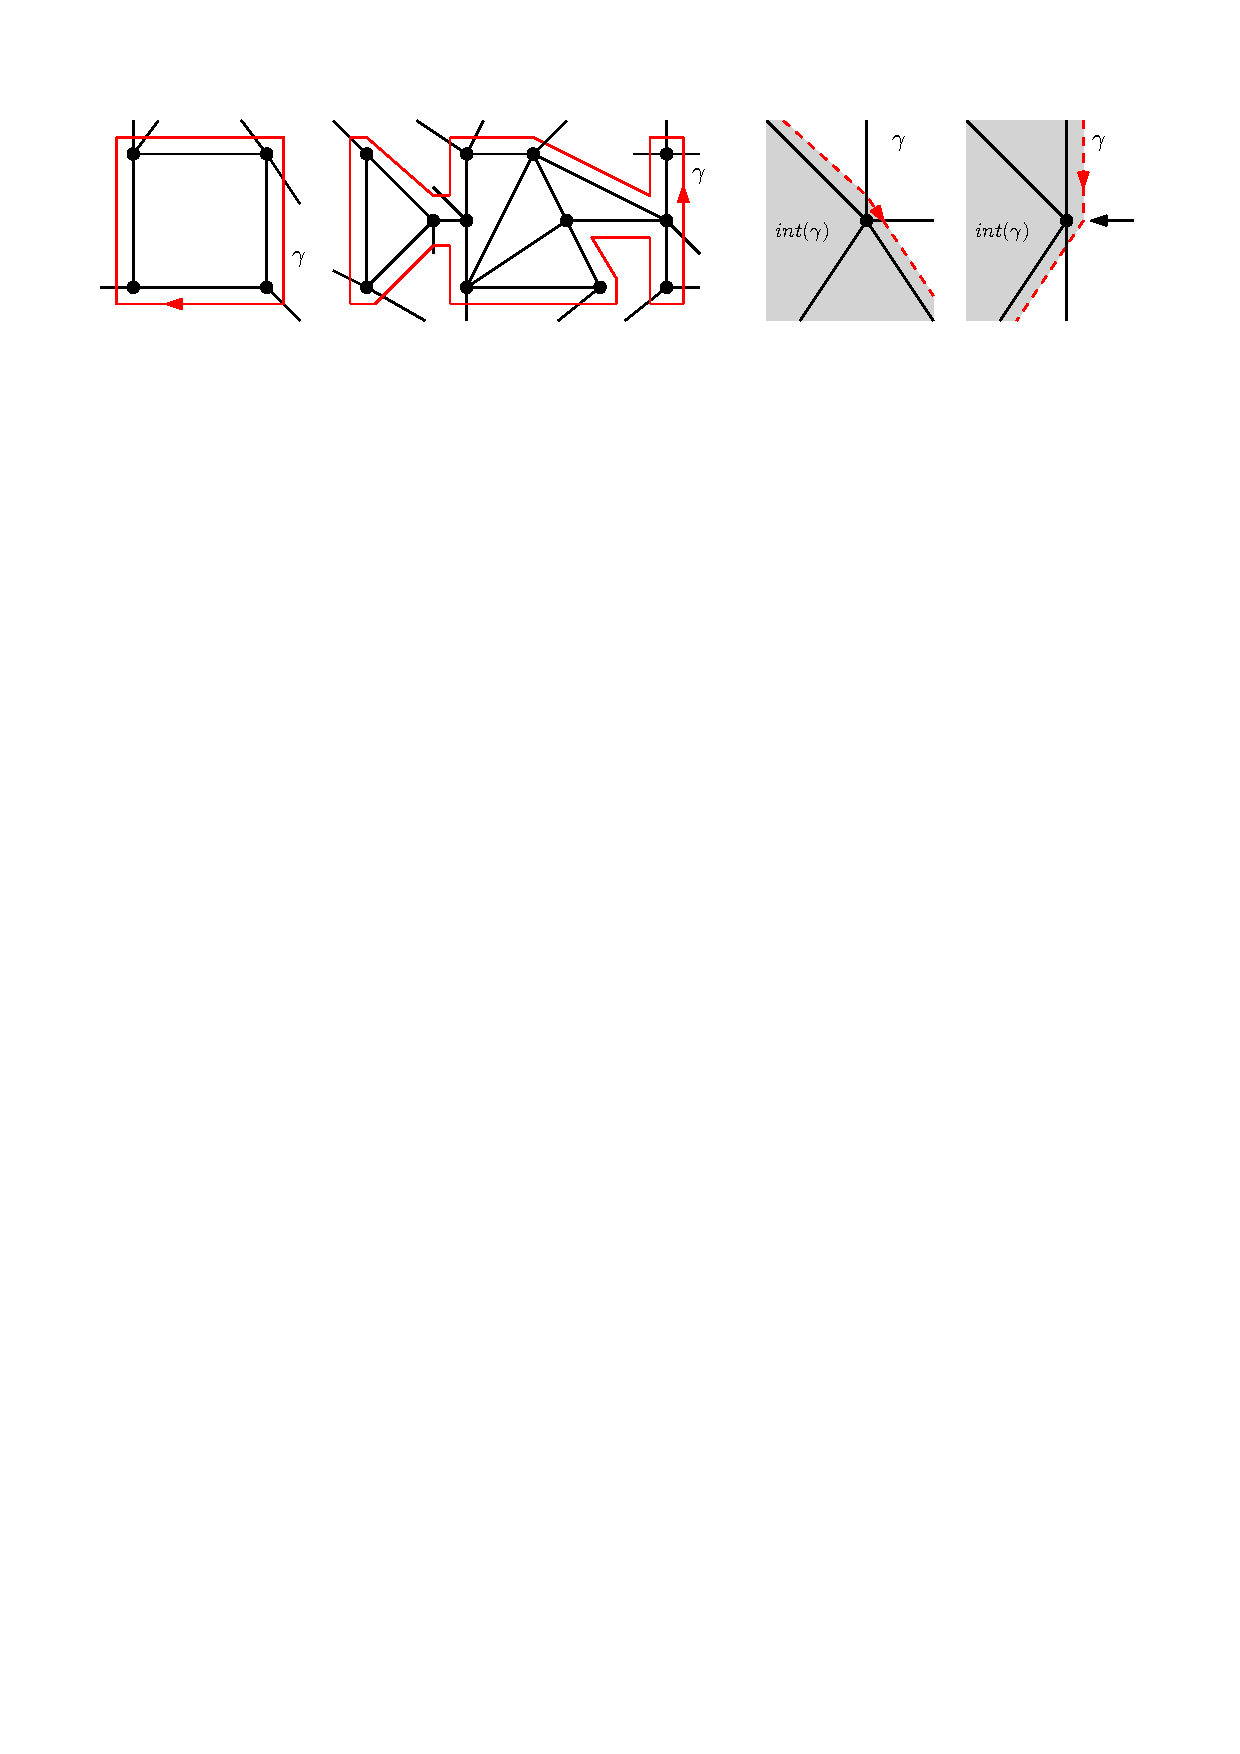
\includegraphics[width=1\textwidth]{corner_def.pdf}
  \caption{Auf der linken Seite zwei Beispiele für \textit{begrenzende Zykel} und rechts für \textit{kombinatorisch konvexe Ecken} mit und ohne zugewiesenem Knoten.}
  \label{corner_def}
\end{figure}

\begin{remark}
Angenommen wir haben einen ebenen Graphen $G$ mit Aufhängungen $\{a_1,a_2,a_3\}$ und ein FAA auf $G$ gegeben. Um aus diesem FAA eine SLTR zu erzeugen, müssen wir die Gebiete in die Form von Dreiecken bringen. Stellen wir uns vor, dass alle Knoten auf einem Haufen liegen. Als Erstes \glqq ziehen\grqq{ }wir die Aufhängungen auseinander, um uns dann Stück für Stück nach innen vorzuarbeiten. Sind wir so bei einem Restgraphen $H$ angekommen, dann brauchen wir mindestens drei Knoten auf Rand, also $\gamma(H)$, an denen wir \glqq ziehen\grqq{ }können, um H in eine konvexe Form zu bringen, ohne dabei einen flachen Winkel des FAA zu verletzten. Kombinatorisch konvexe Ecken entsprechen anschaulich gesehen diesen Knoten.
\end{remark}

\begin{example}
Betrachten wir eine SLTR und einen begrenzenden Zykel $\gamma$, der nicht von einem Pfad induziert wird. In Abbildung \ref{pic_exp_cycle} ist so eine SLTR mit dem begrenzenden Zykel in rot abgebildet. Sei $K$ die konvexe Hülle von $\gamma$ in der SLTR. Sie ist hier grau unterlegt. Dann muss jede Ecke von $K$ einen Außenwinkel haben, welcher grösser als $\pi$ ist. Und da $K$ nicht von einem Pfad induziert ist, müssen mindestens drei Ecken existieren (die drei roten Kreise). Es handelt sich um geometrisch konvexe Ecken in der SLTR. Nun ist der Knoten $v$ an dieser Ecke entweder eine Aufhängung (wie unten links) oder es muss eine Kante geben, die $K$ verlässt, denn in einer SLTR kann kein Winkel (ausser an den Aufhängungen) grösser sein als $\pi$. Wenn der Knoten $v$ an der Ecke keine Aufhängung ist, dann existiert also mindestens eine Kante $(v,w) \notin K$. Es handelt sich also bei $v$ auch um eine kombinatorisch konvexe Ecken von $\gamma$. Somit hat $\gamma$ mindestens drei kombinatorisch konvexe Ecken in der SLTR. 
\end{example}

\begin{figure}[h]
	\centering
  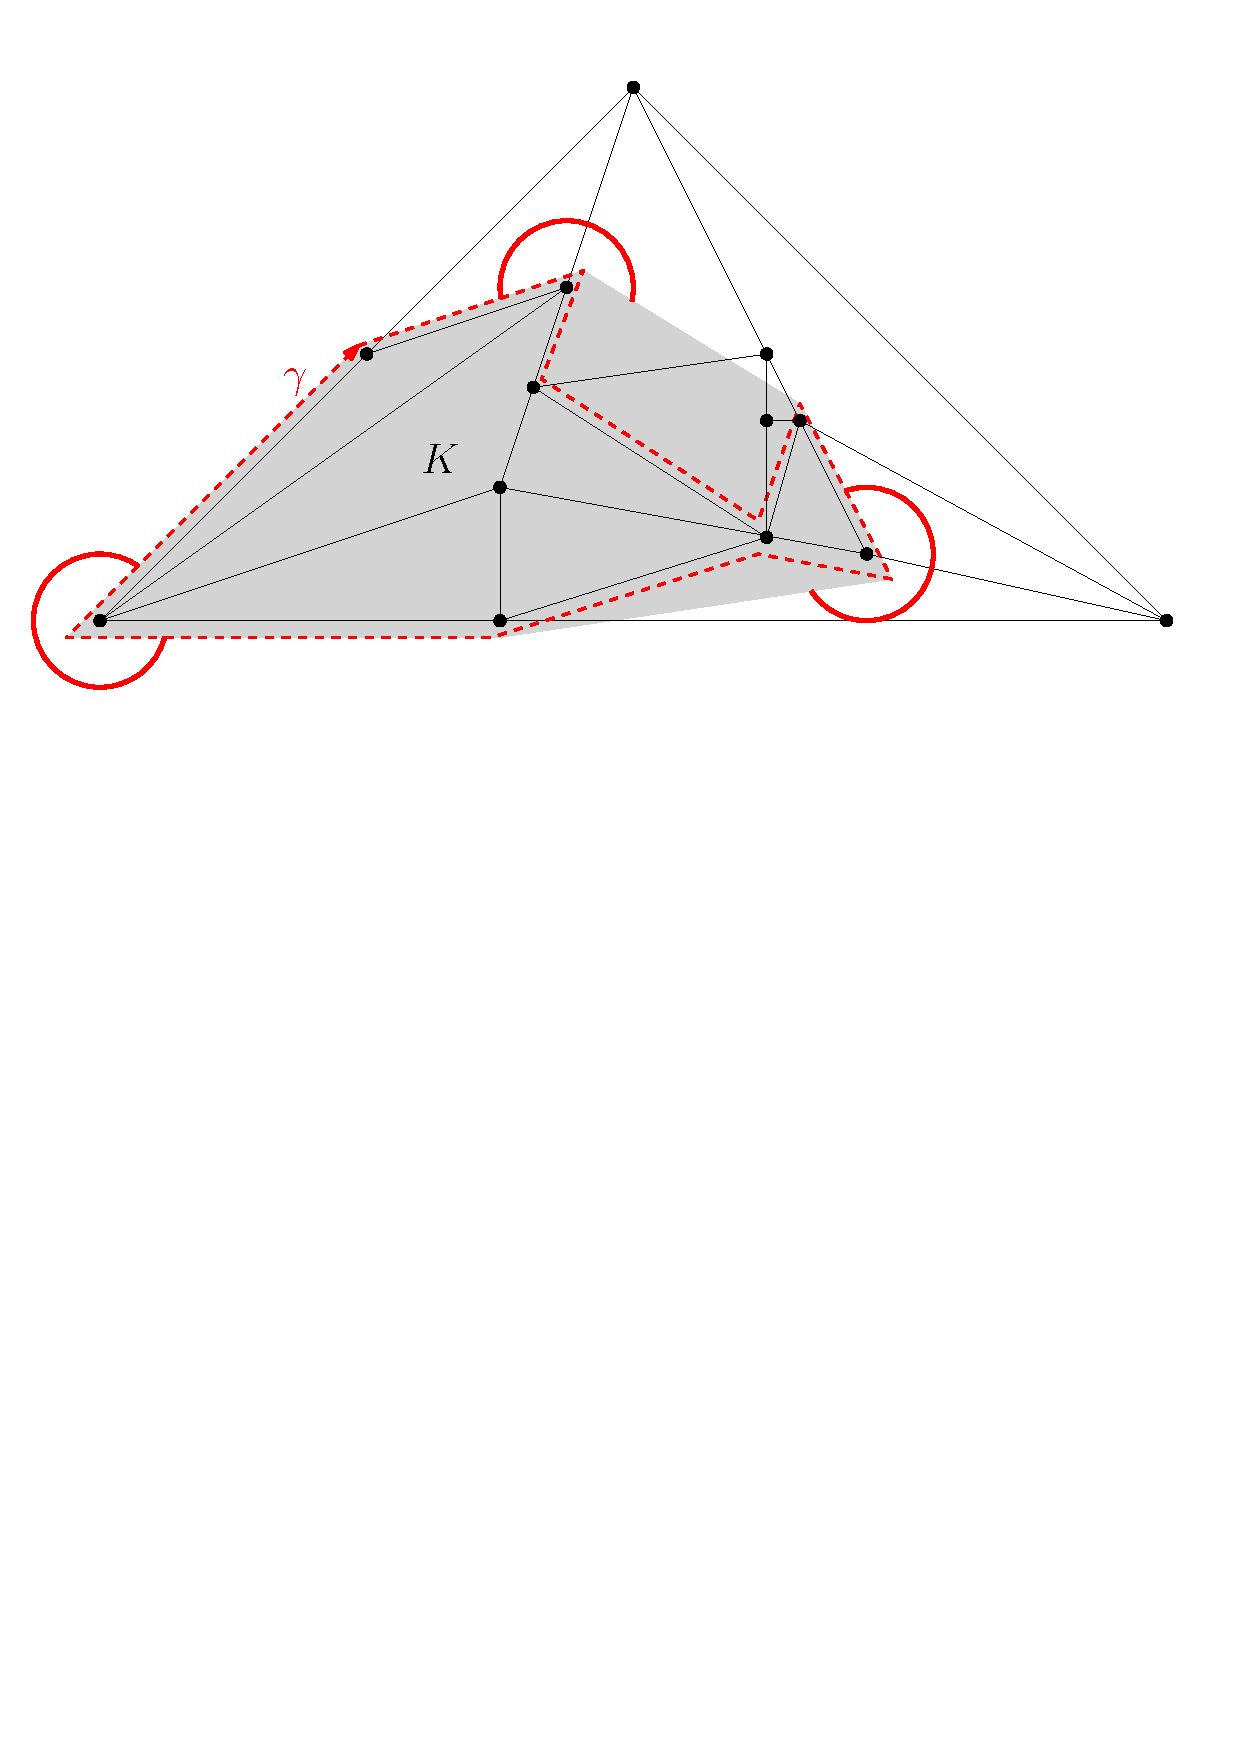
\includegraphics[width=0.7\textwidth]{exp_cycle.pdf}
  \caption{Eine SLTR eines Graphen mit einem begrenzenden Zykel $\gamma$ in rot. Die roten Kreise stellen drei geometrisch und kombinatorisch konvexe Ecken von $\gamma$ dar.}
  \label{pic_exp_cycle}
\end{figure}

Die Beobachtung aus dem Beispiel gilt allgemein für SLTRs und begrenzende Zykel. Die folgende Präposition nach \cite[Prop 2.2, Prop 2.4]{af13} hält sie fest:

\begin{proposition}\label{com_prop}
Sei $G$ ein ebener Graph, der eine SLTR zulässt. Sei weiter $\phi$ das von der SLTR induzierte FAA. Sei $H$ ein zusammenhängender Teilgraph von G (kein Pfad) und $\gamma = \gamma(H)$ sein begrenzender Zykel. Falls $v$ eine geometrisch konvexe Ecke von $\gamma$ in der SLTR ist, dann ist $v$ auch eine kombinatorisch konvexe Ecke von $\gamma$ hinsichtlich $\phi$. Somit gilt:
\begin{itemize}
\item [E4] Jeder begrenzende Zykel $\gamma$, der nicht von einem Pfad induziert wird, hat hinsichtlich $\phi$ mindestens drei kombinatorisch konvexe Ecken.
\end{itemize}
\end{proposition}

Proposition \ref{com_prop} liefert also eine notwendige Bedingung, damit ein FAA von einer SLTR induziert sein kann. Dies ist sogar eine hinreichende Bedingung, wie im Verlauf des Kapitels in Theorem \ref{com_theo} gezeigt wird. 

\begin{definition}[Gutes-FAA]
Wir nennen ein FAA, das E4 aus Proposition \ref{com_prop} erfüllt, im Weiteren \textit{Gutes-FAA} oder kurz \textit{GFAA}.
\end{definition}

Aerts und Felsner zeigen, dass ein Gutes-FAA eine \textit{Kontaktfamilie von Pseudosegmenten} induziert, die sich somit geradlinig darstellen lässt. Wir beginnen mit der Definition.

\begin{definition}[Kontaktfamilie von Pseudosegmenten]
Eine \textit{Kontaktfamilie von Pseudosegmenten} ist eine Familie $\Sigma = \{c_i\}_{i\in I}$ von einfachen Kurven $$c_i:[0,1] \to \mathbb{R}^2, \text{ mit } c_i(0) \neq c_i(1),$$ sodass alle Kurven $c_i,c_j$ mit $i \neq j$ maximal einen gemeinsamen Punkt haben. Dieser Punkt muss dann ein Endpunkt von mindestens einer der Kurven sein.
\end{definition}

Ein GFAA $\phi$ liefert eine Relation $\rho$ auf den Kanten von G. Zwei Kanten $(v,w)$ und $(v,u)$, beide adjazent zu $f$, stehen genau dann in Relation, wenn $\phi(v)=f$. $(v,w)$ und $(v,u)$ müssen also auf der selben Seite  des Dreiecks $f$ in der SLTR liegen. Der transitive Abschluss dieser Relation liefert eine Äquivalenzrelation $\rho$. Die Aquivalenzklassen von $\rho$ bilden eine Kontaktfamilie von Pseudosegmenten.

Nennen wir die Äquivalenzklassen von $\rho$ Kurven, dann gilt nach F2, dass jeder Knoten nur einem Gebiet zugeordnet werden kann und somit auch nur im Inneren von einer Kurve liegt. Die Kurven können sich also nicht kreuzen, sondern es kann nur eine an einer anderen enden. Weiter hat jede Kurve unterschiedliche Anfangs- und Endpunkte und kann sich nicht selbst berühren. Dies kann man so begründen, dass sonst der resultierende begrenzende Zykel $\gamma$ nur eine, beziehungsweise zwei kombinatorisch konvexe Ecken hätte. Das wäre ein Widerspruch zu E4. Analog können zwei Kurven nicht ihre Anfangs- und Endpunkte teilen, da sonst wieder ein Zykel mit zu wenigen Ecken entstehen würde. Für eine von einem FAA $\phi$ induzierte Kontaktfamilie schreiben wir auch $\Sigma_{\phi}$. 

\begin{figure}[h]
	\centering
  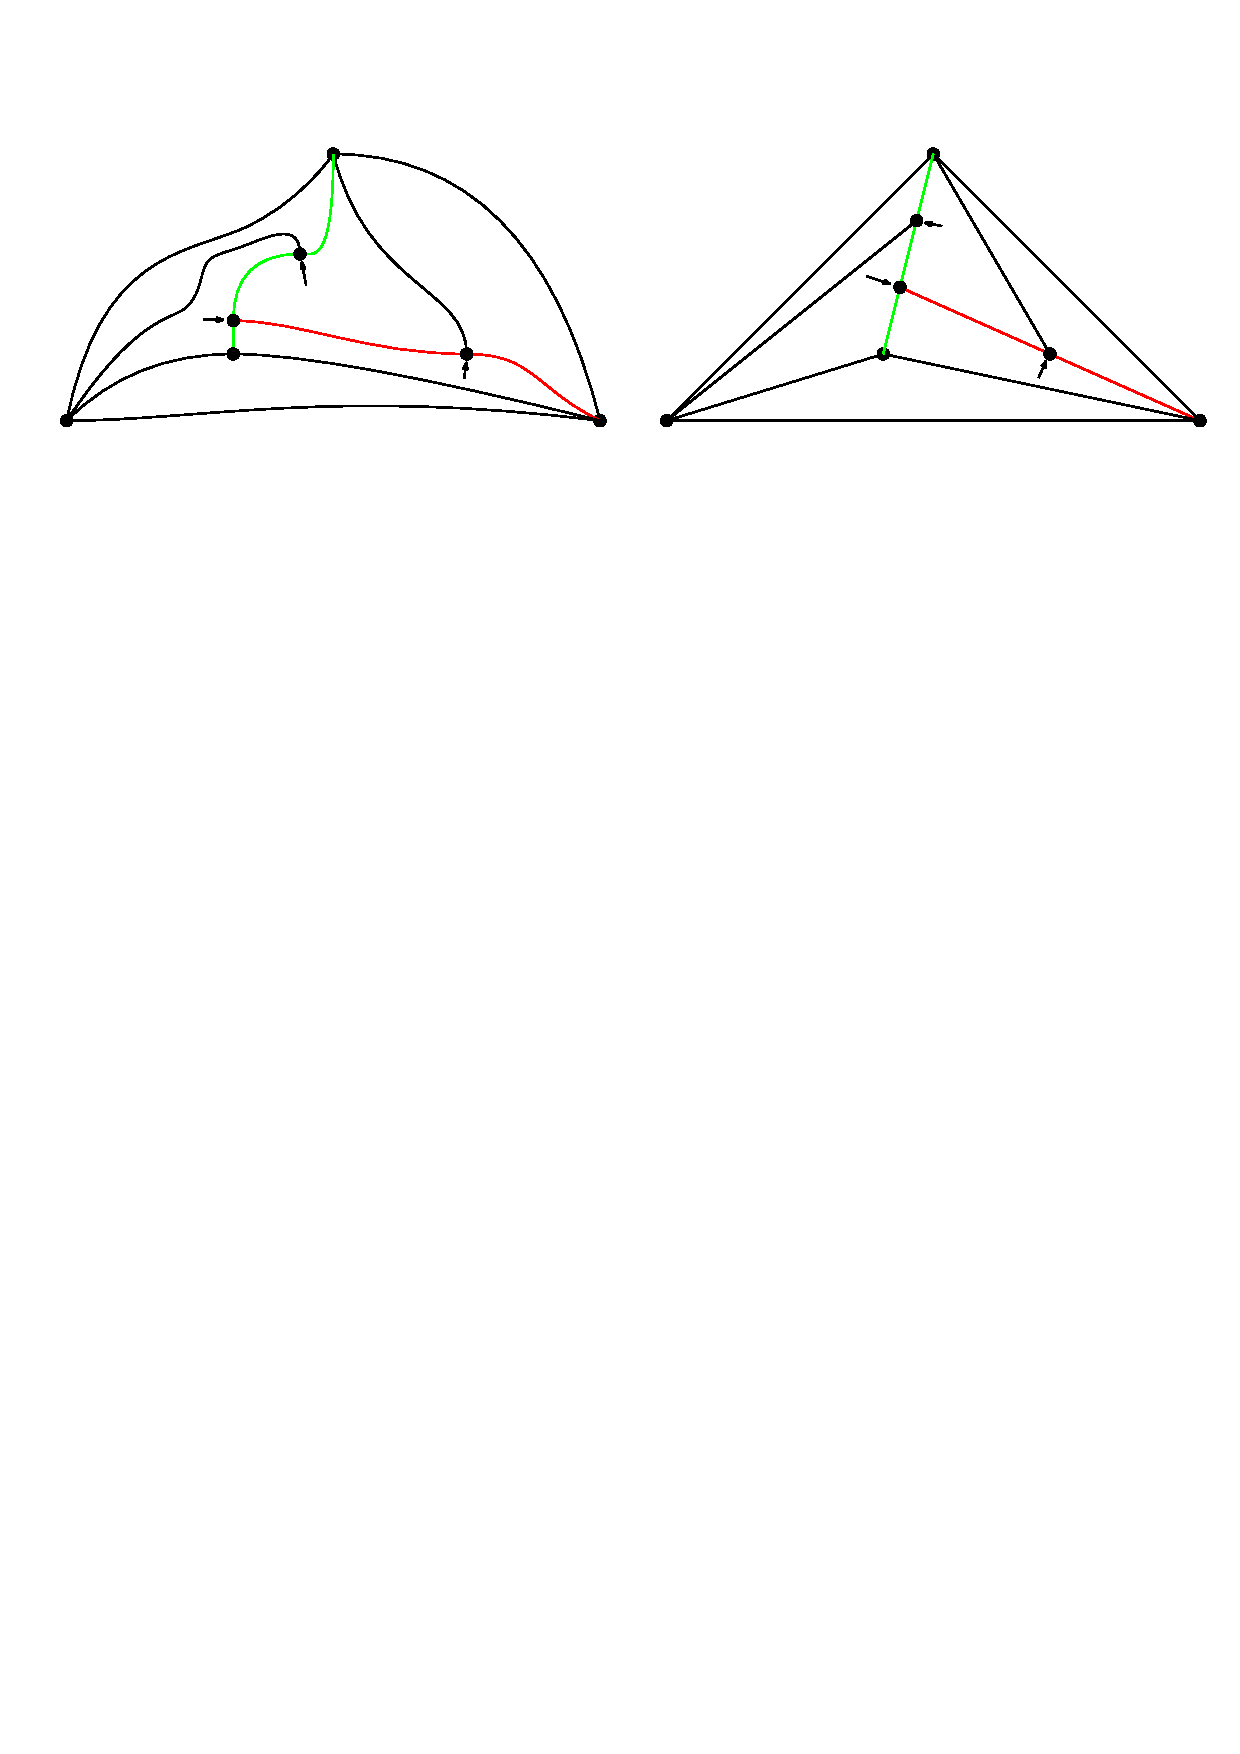
\includegraphics[width=1\textwidth]{pseudo_seg.pdf}
  \caption{Die Kanten von G als Kontaktfamilie von Pseudosegmenten induziert durch die Äquivalenzrelation. In rot und grün die beiden Äquivalenzklassen bzw. Kurven, die mehr als eine Kante beinhalten.}
\end{figure}

\begin{definition}
Sei $\Sigma$ ein Kontaktfamilie von Pseudosegmenten und $S\subseteq\Sigma$. Wir nennen einen Punkt $p\in S$ einen \textit{freien Punkt}, falls er die folgenden Bedingungen erfüllt.
\begin{itemize}
\item p ist ein Endpunkt eines Pseudosegmentes aus S.
\item p liegt nicht im Inneren eines Pseudosegmentes aus S.
\item p liegt am äußeren Rand von S.
\item p ist entweder eine Aufhängung von G oder berührt ein Pseudosegment, welches nicht zu S gehört.
\end{itemize} 
\end{definition}

\begin{figure}[h]
	\centering
  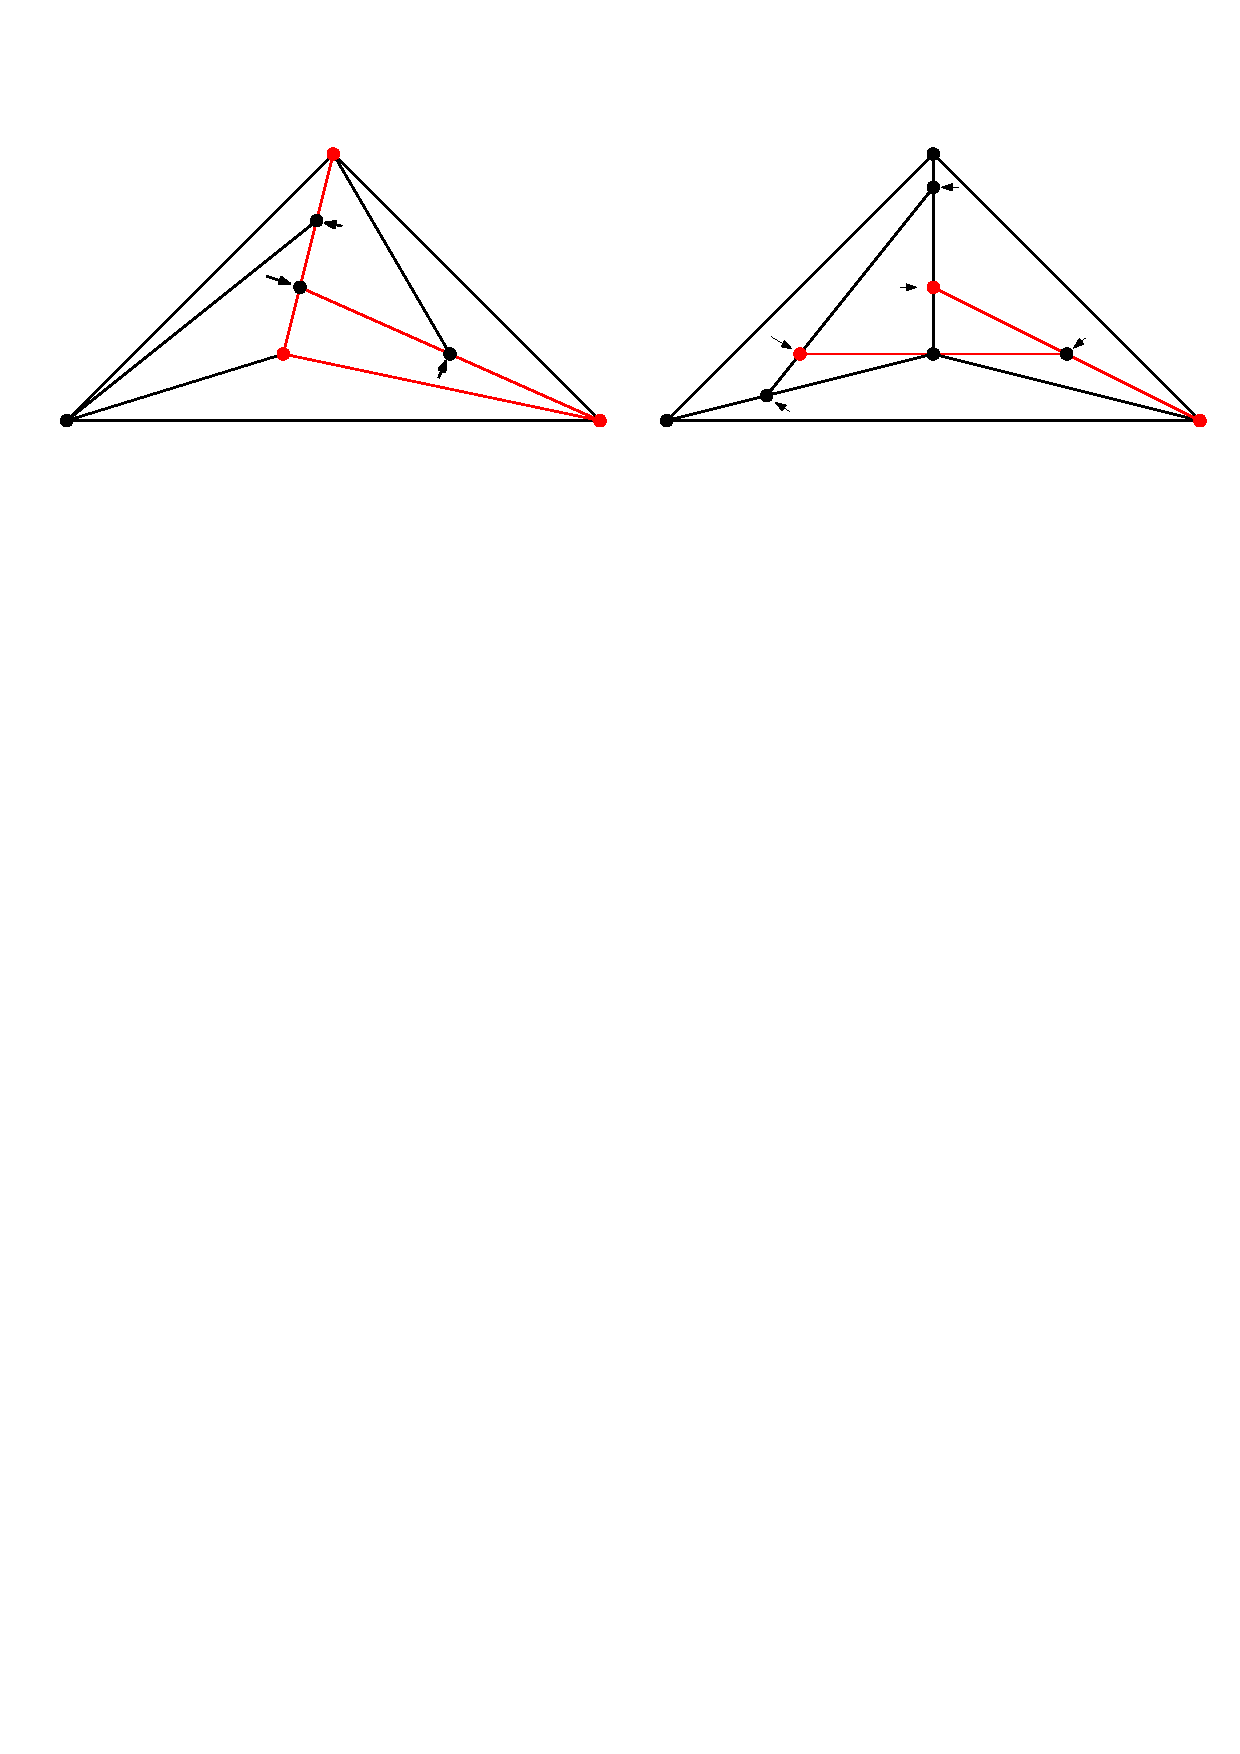
\includegraphics[width=1\textwidth]{exp_free.pdf}
  \caption{Zwei SLTRs mit Teilfamilien von Pseudosegmenten in rot und den freien Punkten dieser Familien ebenfalls in rot.}
\end{figure}

\begin{lemma}\cite[Lemma 2.8]{af13}\label{lemma_af13}
Sei $\phi$ ein Gutes-FAA auf einem ebenen und intern 3-zusammenhängenden Graphen, dann gilt: 
\begin{itemize}
\item [E5] Jede Teilmenge $S \subseteq \Sigma_{\phi}$ mit $|S| \geq 2$ hat mindestens 3 freie Punkte.
\end{itemize}
\end{lemma}

Betrachte einen ebenen, intern 3-zusammenhängenden Graphen $G$ mit Aufhängungen $\{a_1,a_2,a_3\}$ und einem GFAA $\phi$. Wenn die von $\phi$ induzierte Kontaktfamilie $\Sigma_{\phi}$ mit geradlinigen Segmenten darstellbar ist, dann ist diese Darstellung eine zu $\phi$ passende SLTR für $G$. Für den Fall, dass eine solche Darstellung $f:G\to\mathbb{R}^2$ existiert, können für die Koordinaten der Segmente oder genauer für die Knoten $v$ von $G$ auf den Segmenten im Folgenden Gleichungen aufgestellt werden. Die Positionen $f(v)$ der Knoten $v$ in der Einbettung $f(G)$ müssen diese Gleichungen erfüllen. Das resultierende Gleichungssystem beinhaltet harmonische Funktionen. Bevor wir die Gleichungen, die unser Problem charakterisieren, in Abschnitt \ref{the_equations} angeben, werden wir zu harmonischen Funktionen einen kurzen Überblick geben.

\subsection{Harmonische Funktionen auf planaren Graphen}

Die Theorie zu (diskreten) harmonischen Funktionen auf planaren Graphen und ihre Anwendung wird in \cite{lov99} ausführlich behandelt. Es handelt sich um eine Diskretisierung von allgemeinen harmonischen Funktionen, also glatten Funktionen $f:G\subseteq \mathbb{R}^n \to \mathbb{R}$, mit $\Delta f = 0$, wobei $\Delta$ den Laplace Operator beschreibt. Für diese Funktionen gilt, dass der Funktionswert an einem Punkt $x$ dem Durchschnitt der Funktionswerte auf einem Ball um $x$ entspricht. 

Dies führt zu der folgenden Definition im diskreten Fall.

\begin{definition}[Harmonische Funktionen]
Sei $G=(V,E)$ ein planarer zusammenhängender Graph und $S \subseteq V$. Eine Funktion $g:V \to \mathbb{R}$ nennen wir am Knoten $v \in V$ \textit{harmonisch}, falls gilt:
$$ \text{H1} \quad \sum_{u \in N(v)}(g(u) - g(v)) = 0 \quad \qquad\qquad \qquad\qquad\qquad\qquad\qquad\qquad\qquad\quad\:\,\:$$
Wir können H1 durch das Hinzufügen einer nichtnegativen Gewichtsfunktion $\lambda:E\to\mathbb{R}_+$ verallgemeinern. Es gilt $\lambda(v,w) = \lambda_{vw}$.
$$ \text{H2}\quad \sum_{u \in N(v)}\lambda_{uv}(g(u) - g(v)) = 0 \quad\qquad \qquad\qquad \qquad\qquad\qquad\qquad\qquad\qquad$$
Einen Knoten, für den $g$ nicht harmonisch ist, nennen wir \textit{Pol}.
\end{definition}

\begin{theorem}\cite[Theorem 3.1.2]{lov99}\label{harmonic_uni}
Für jede nichtleere Teilmenge $S \subseteq V$ und jede Funktion $g_S:S\to\mathbb{R}$ existiert genau eine Funktion $g:V\to\mathbb{R}$, die $g_S$ auf $V$ fortsetzt, sodass $g$ in jedem Knoten $v\in V \backslash S$ harmonisch ist. Wir nennen sie die harmonische Fortsetzung von $g_S$ auf $V$.
\end{theorem}

Ein bekanntes Resultat, das sich in Form harmonischer Funktionen darstellen lässt, ist Tuttes \textit{rubber-band-representation}, die konvexe Zeichnungen für planare Graphen liefert \cite{tutte63}. Man stelle sich einen planaren Graphen vor, bei dem jede Kante durch ein idealisiertes Gummiband\footnote{Die Gummibänder müssen das Hook'sche Gesetzt erfüllen, sodass eine Streckung auf Länge $l$ genau Kraft $l$ benötigt.} ersetzt wird. Fixiere für den Moment alle Knoten in einem beliebigen Punkt. Wähle nun ein äußeres Gebiet $f_{aus}$. Die Menge $S\subseteq V$ seien die zu $f_{aus}$ adjazenten Knoten. Nun fixieren wir diese Knoten in zyklischer Reihenfolge und in gleichen Abständen auf einem Kreis in der Ebene. Dies definiert $f_x:S \to \mathbb{R}$ und  $f_y:S \to \mathbb{R}$. Wenn wir nun die restlichen Knoten loslassen, dann werden sie von den Gummibändern in eine neue Position gezogen. Das resultierende Gleichgewicht, das genau dann entsteht, wenn H1 für beide Komponenten von $f$ erfüllt ist, entspricht der (komponentenweisen) harmonischen Fortsetzung von $f=(f_x,f_y)$  auf $V$, wobei $f(v)$ genau der Position von $v$ in der resultierenden Einbettung entspricht und $S$ die Menge der Pole von $f$ ist. Wir können die Kanten zusätzlich noch mit nicht negativen Gewichten $\lambda_{vw}$, versehen, um die Einbettung zu verändern. Das folgende Theorem ist das Hauptresultat dieser Vorgehensweise \cite{tutte63}.

\begin{theorem}\label{theo_rubber}
Sei $G$ ein planarer Graph, dann ist eine \textit{Gummiband-Representation (rubber-band-representation)} von $G$ eine planare Einbettung in der Ebene.
\end{theorem}

\subsection{Das resultierende Gleichungssystem}\label{the_equations}

Die Theorie zu harmonischen Funktionen lässt sich auf SLTRs anwenden. Sei $G$ ein planarer Graph und $\phi$ ein FAA. Nehme für den Moment an, es existiert eine geradlinige Darstellung der Pseudosegmente $\Sigma_{\phi}$. Wir haben also eine geradlinige Einbettung $f(G)$ der von $\phi$ induzierten Segmente. 

Es gilt für jeden Knoten $v$ im Inneren eines Segmentes, also für jeden zugewiesenen Knoten, dass er auf einer Gerade zwischen seinen beiden benachbarten Knoten $u,w$ auf dem Segment liegen muss. Diese Eigenschaft liefert die komponentenweisen Bedingungen 
\begin{equation}\label{harm_1}
\begin{split}
f_x(v) &= \lambda_v f_x(u) + (1-\lambda_v)f_x(w) \text{, mit } \lambda_v \in (0,1)\\
f_y(v) &= \lambda_v f_y(u) + (1-\lambda_v)f_y(w) \text{, mit } \lambda_v \in (0,1).
\end{split}
\end{equation}
Für die nicht zugewiesenen Knoten aus $G$ muss in einer SLTR gelten, dass sie sich in der konvexen Hülle ihrer Nachbarn befinden. Wir bilden einen (gewichteten) Schwerpunkt und erhalten komponentenweise 
\begin{equation}\label{harm_2}
\begin{split}
f_x(v) &= \sum_{u \in N(v)} \lambda_{uv} f_x(u) \text{, mit }  \sum_{u \in N(v)}\lambda_{uv} = 1 \text{ und } \lambda_{uv} \geq 0.\\
f_y(v) &= \sum_{u \in N(v)} \lambda_{uv} f_y(u) \text{, mit }  \sum_{u \in N(v)}\lambda_{uv} = 1 \text{ und } \lambda_{uv} \geq 0.
\end{split}
\end{equation}

Somit erfüllt die so gegebene Funktion $f:V\to\mathbb{R}^2$ mit $f=(f_x,f_y)$ und passend gewählten $\lambda$ wegen (\ref{harm_1}) und (\ref{harm_2}) in beiden Komponenten H2. Es handelt sich somit bei $f_x$ und $f_y$ um harmonische Funktionen mit den Polen $\{a_1,a_2,a_3\}$. Nach Theorem \ref{harmonic_uni} existiert für jede, den Beschränkungen entsprechende Wahl von $\lambda$, somit genau eine Funktion $f=(f_x,f_y)$, welche die Gleichungen \ref{harm_1} und \ref{harm_2} erfüllt.

Dies führt uns zum Hauptresultat aus \cite{af13}:

\begin{theorem}\label{com_theo}
Sei $G$ ein intern-3-zusammenhängender, ebener Graph und $\Sigma$ eine Familie von Pseudosegmenten, induziert von einem FAA, sodass jede Teilfamilie $S \subset \Sigma$ entweder mindestens drei freie Punkte hat oder maximal ein Element enthält. Dann induziert die eindeutige Lösung $f:V\to \mathbb{R}^2$ des aus $\Sigma$ resultierenden Gleichungssystems eine SLTR. 
\end{theorem}

\begin{remark}
Dies bedeutet, dass die notwendigen Bedingungen E4 und E5, die in Lemma \ref{lemma_af13} und in Proposition \ref{com_prop} festgehaltenen wurden, auch hinreichende Bedingungen sind. Falls wir schon ein Gutes-FAA gefunden haben, dann können wir mit Hilfe des obigen Ansatzes auch eine Einbettung in der Ebene erhalten. Es gilt jedoch für viele Graphen, dass sie, wie in Beispiel \ref{bsp_exp_faa}, exponentiell vielen FAAs besitzen. Selbst wenn wir die hinreichende Bedingung E4 in polynomineller Zeit überprüfen könnten, erreichen wir auf diesem Weg keinen schnellen Algorithmus.
\end{remark}

Aerts und Felsner werfen am Ende von \cite{af13} die Frage nach einer guten Wahl von $\lambda$ auf und wie dies die resultierenden Einbettungen beeinflussen kann. Kapitel \ref{the_program} wird einer möglichen Antwort dieser Frage nachgehen.

\begin{figure}
	\centering
  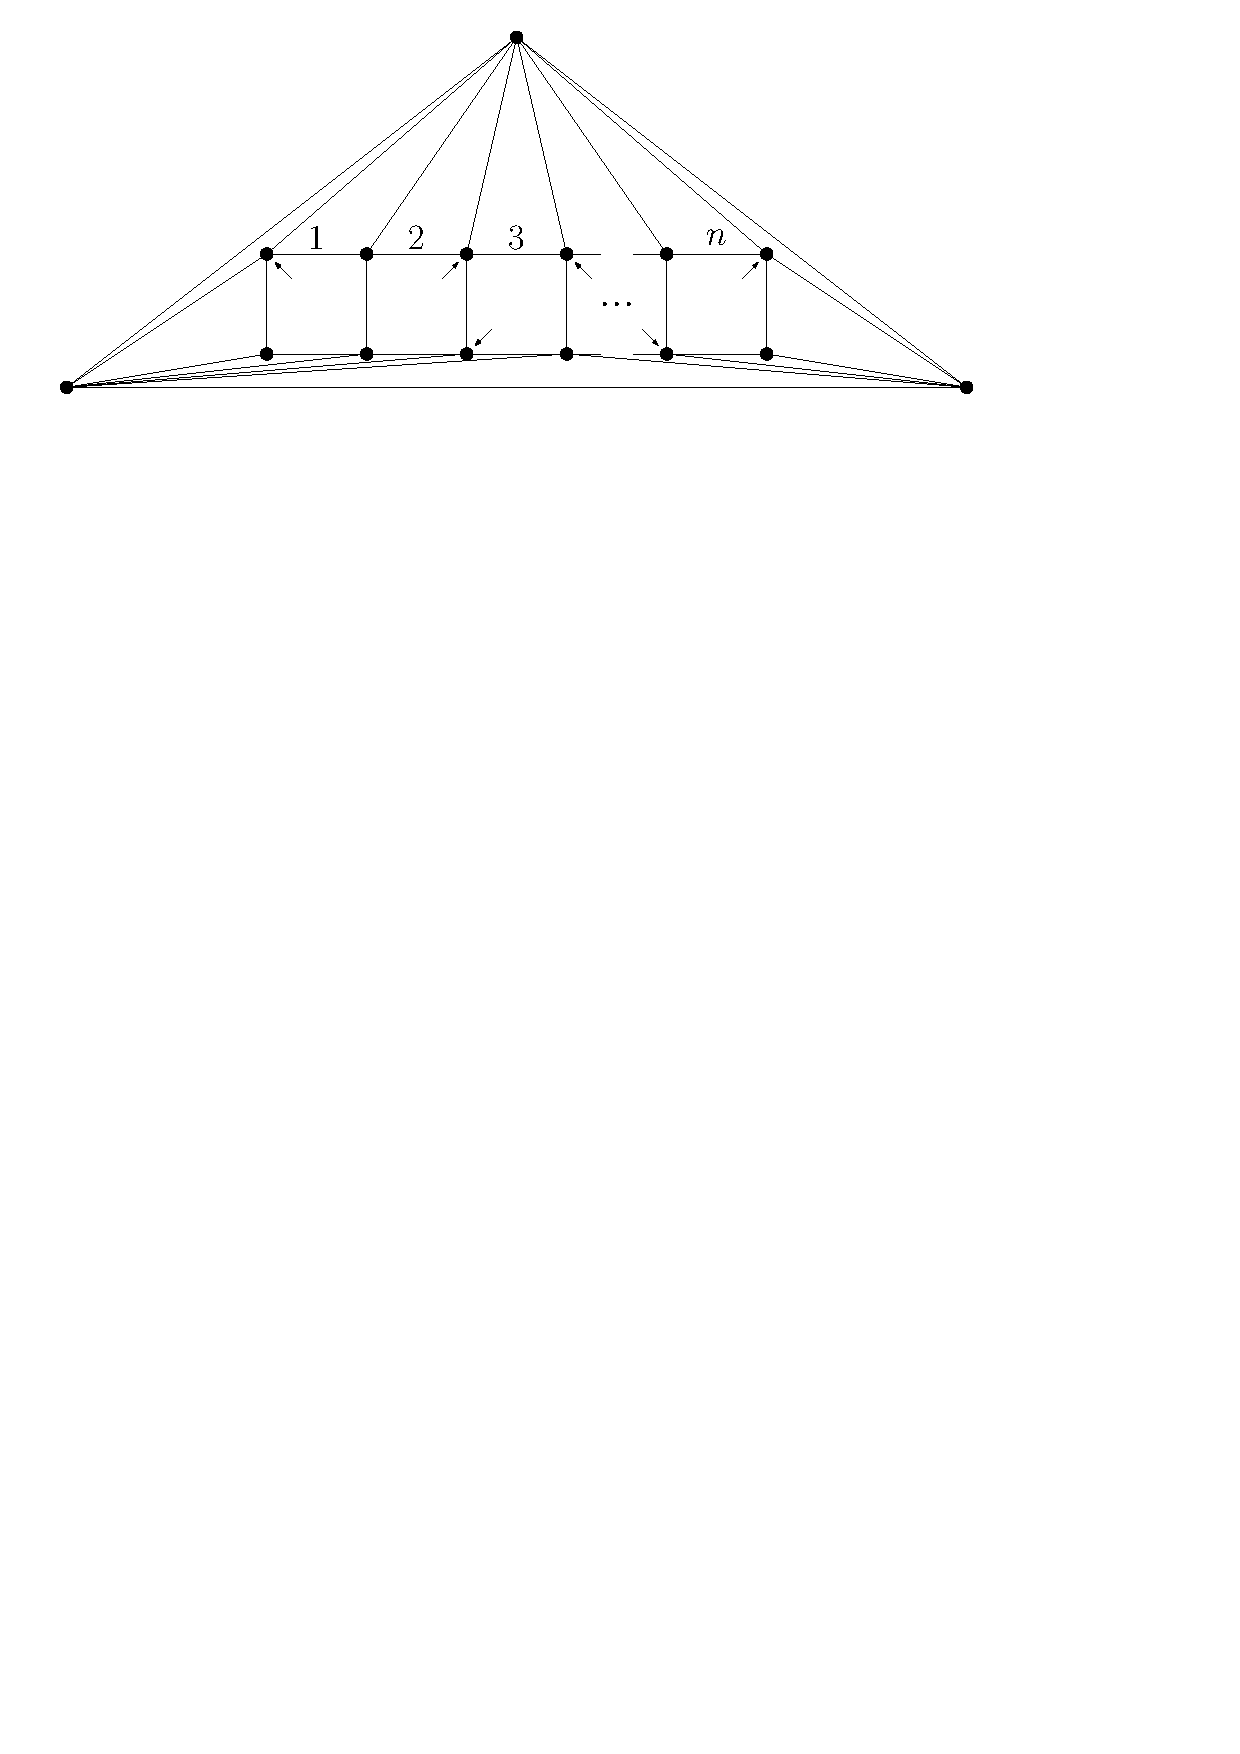
\includegraphics[width=0.7\textwidth]{exp_faa.pdf}
  \caption{Ein Graph mit exponentiell vielen FAAs.}
  \label{exp_faa}
\end{figure}

\begin{example}\label{bsp_exp_faa}
Betrachten wir eine zusammenhängende Kette von $n$ Quadraten in der Ebene und verbinden wir ihre Eckpunkte mit drei Aufhängungen $a_1,a_2,a_3$, welche ein Dreieck bilden. Der so erzeugte Graph $G$ hat $2n+5$ Knoten und ist in Abbildung \ref{exp_faa} zu sehen. Wir wollen nun ein FAA für diesen Graphen erstellen (welches nicht zwangsläufig eine SLTR zulässt). Wir müssen für ein FAA jedem der inneren Quadrate einen Winkel zuordnen. Wenn wir von links beginnen und nach rechts laufen, können wir in jedem der $n$ inneren Quadrate mindestens aus drei Winkeln auswählen, um ein FAA zu erstellen. Es wurde höchstens einer der beiden Knoten auf der linken Seite von Quadrat $i$ im Schritt zuvor zugewiesen. Somit existieren mehr als $3^n$ FAAs für $G.$
\end{example}
